\documentclass[10pt,twocolumn,letterpaper]{article}

\usepackage{cvpr}
\usepackage{times}
\usepackage{epsfig}
\usepackage{graphicx}
\usepackage{amsmath}
\usepackage{amssymb}
\usepackage{verbatim}

% Include other packages here, before hyperref.

% If you comment hyperref and then uncomment it, you should delete
% egpaper.aux before re-running latex.  (Or just hit 'q' on the first latex
% run, let it finish, and you should be clear).
\usepackage[breaklinks=true,bookmarks=false]{hyperref}

\cvprfinalcopy % *** Uncomment this line for the final submission

\def\cvprPaperID{****} % *** Enter the CVPR Paper ID here
\def\httilde{\mbox{\tt\raisebox{-.5ex}{\symbol{126}}}}

% Pages are numbered in submission mode, and unnumbered in camera-ready
%\ifcvprfinal\pagestyle{empty}\fi
%\setcounter{page}{4321}
\begin{document}

%%%%%%%%% TITLE
\title{Facial Keypoints Detection Using Convolutional Neutral Network}

\author{Qinyao He\\
CST34\\
Tsinghua University\\
{\tt\small 2012010548}
% For a paper whose authors are all at the same institution,
% omit the following lines up until the closing ``}''.
% Additional authors and addresses can be added with ``\and'',
% just like the second author.
% To save space, use either the email address or home page, not both
\and
Xiaocheng Yang\\
CST34\\
Tsinghua University\\
{\tt\small 2013011383}
}

\maketitle
%\thispagestyle{empty}

%%%%%%%%% ABSTRACT
\begin{abstract}
   In this report we building an neural network for carrying out facial
   keypoints detection problem. We have tried several ways, but a problem
   of non convergence still need to be resolved, which till now we have no
   idea about that.
\end{abstract}

%%%%%%%%% BODY TEXT
\section{Introduction}

This task comes originally from Kaggle\footnote{https://www.kaggle.com/},
a online website holding many data science competitions. It's aim is to
determine the location of several certain key points on face, given a photograph
contains a human face.

This key points detection can form the building block for many applications. Such as:
	\begin{itemize}
		\item[*] tracking faces in images and video
		\item[*] analysing facial expressions
		\item[*] detecting dysmorphic facial signs for medical diagnosis
		\item[*] biometrics / face recognition
	\end{itemize}
Detecing facial keypoints is a very challenging problem. 
Facial features vary greatly from one individual to another,
and even for a single individual, there is a large amount of variation
due to 3D pose, size, position, viewing angle, and illumination conditions.
Computer vision research has come a long way in addressing these difficulties,
but there remain many opportunities for improvement.

In this specific competition\footnote{https://www.kaggle.com/c/facial-keypoints-detection}, 
we are required to localize 15 facial key points given a images. Each predicted point
is specified as $(x,y)$ real-valued pair in the space of pixel indices.
The 15 keypoints is: 

left\_eye\_center, right\_eye\_center, left\_eye\_inner\_corner, left\_eye\_outer\_corner, right\_eye\_inner\_corner, right\_eye\_outer\_corner, left\_eyebrow\_inner\_end, left\_eyebrow\_outer\_end, right\_eyebrow\_inner\_end, right\_eyebrow\_outer\_end, nose\_tip, mouth\_left\_corner, mouth\_right\_corner, mouth\_center\_top\_lip, mouth\_center\_bottom\_lip

so 30 real value is going to be predicted for each input image.

Kaggle given a training data set of 7049 image with size of $96*96$,
color is gray scale and represented as an integer from 0 to 255 for each
pixel. And each training images is labeled with 30 real value for position of the 
15 key points. In some examples, some of the target keypoint positions are misssing.

Also, a test set of 1783 images without label is given, for competitors to submit their
predicted result to Kaggle for score.

Performance is graded by MSE(mean square error) for those 30 real values. A lower
MSE indicate a better prediction.

In our work, we have carried out experiment on several models, include basic multilayer
perceptron, convolutional neural network and cascaded convolutional network.


\section{Related Work}
Same problem have already been addressed as course project by two student in
Stanford University\cite{wangfacial}. They only detect two key point among those 15
points given, which is left\_eye\_center and right\_eye\_center, and this two points are
relatively easy to detect.

They use a traditional machine learning method. They first do data normalization on
the brightness of each image, set the brightest point to 255 and the darkest point to 0.
Then perform a principle component analysis on the data set to find several \emph{eigen face}.
Last use a \emph{Mean Patch Searching} to find the position.

They obtain a MSE of 2.88 on the two key points.

Another work using convolutional neural network is by Sun, Yi\cite{sun2013deep} use three
convolutional network and cascade them to refine the prediction step by step, using the area
centered by previous layer prediction for refine learning to grasp local structures. They claim to
be the state-of-art work in that time.

\section{Technical Approach}
In this section we demonstrate some technical approach which, based on previous
work, can improve performance of the network, accelerate convergence, and reduce
overfitting.

\subsection{Data Normalization}
In the original training data, each pixel is represented by an integer from 0 to 255,
and the real-value label range from 0 to 96. This large range of input and target data
may force the neuron to saturate, which slow down convergence. Also, the non-error-centered
target value make the full connected layer hard to get a ideal output.

In our implementation, gray scale from 0 to 255 are divided by 256, rescaled to range 0 to 1,
and target value are rescaled and zero centered to range from -1 to 1. Let train\_x, train\_y
stand for the image data and label, the normalize preprocess looks like:
$$
	\begin{aligned}
		train\_x &= \frac{train\_x}{256.0} \\
		train\_y &= \frac{train\_y - 48.0}{48.0}
	\end{aligned}
$$

\subsection{ReLU Nonlinearity}
When training deep feedforward neural network, gradient diminishing when back propagation
often occurs and make it very slow to converge. This issue is common when using sigmoid-like
activation function, since they have a so-called saturation regime where gradient almost vanished.
According to experiment by Glorot \cite{glorot2010understanding}, for a feedforward neural net
with 4 layers and activate with sigmoid function, the last hidden layer quickly saturate with
output value of 0, which slow down the progress of learning. and after a hundred of epochs,
it escaped, and the followed layer began to saturate.

Glorot hypothesize that this behavior is the result of combination of random initialization
and the fact that an output of zero correspond to a saturated sigmoid. Unsupervised pre-training
can successfully solve this issue.

While with another kind of activation function, known as ReLU(rectify linear unit), the problem
of saturation and gradient diminishing is also solved. ReLU activation act as follow:

$$
rectify(x) = max(x, 0)
$$

It can achieve the performance as better
as a pre-trained sigmoid network\cite{glorot2011deep} without any unsupervised pre-training.
It behavior is also more plausible at the viewpoint of biological neural science, which claim
a neuron to be closed below zero, and behave linearly when input is above zero with in some range,
and this range is satisfied most of time.

Also rectifier activation function allow a network to easily obtain sparse representations, which
is biologically plausible and have mathematical advantages.

The non-linearity when using rectify comes from path-selection. For different input, different
set of neurons are active. This model can be viewed as an \emph{exponential
number of linear models that share parameters}\cite{nair2010rectified}.

Experiment shows both improvement on learning speed and performance
\cite{krizhevsky2012imagenet, glorot2011deep}.

In our model, both the convolution layer and the full connected layer is activate by ReLU function
except for the last layer, which followed by the finally loss layer. Because we want the output
result to have both positive and negative value, while ReLU only result in positive and zero.

Also this approach can be used in classification problem with softmax and cross entropy loss.
Allow result to be negative increase the difference when doing softmax, which result in better
classification result.

\subsection{Weight Initialization}
In a deep enough neural network, initialization of weight parameter sometimes determine whether the
training progress converge. A too large initialization cause saturation in case of sigmoid or hyperbolic
activation function, or layer-by-layer amplification of output which finally result in
infinity for NaN when deep enough in case of ReLU. Both case put a obvious obstacle on gradient
descent progress. While too small initialization result in small gradient to propagate
(since this gradient is proportional to the value of the weights).

Typical method is to initialize weights from zero-centered normal or uniform distribution with specified
standard deviation. The choose of this variance, as a hyper-parameter, becomes a problem.
Glorot\cite{glorot2010understanding} propose a method, which commonly called "Xavier" initialization,
based on the assumption that the activations are linear. It take the form:
$$
Var(w) = \frac{2}{n_{in}+n_{out}}
$$
where $n_{in}$ and $n_{out}$ are the number of units in the previous layer and the next layer.
Or equivalently, $n_in$ is the number of input for each neuron, and $n_out$ is the total number of
neuron in this layer.

A more recently research by He\cite{he2015delving} provide a more refined analysis specifically
on ReLU activation, and it has form:
$$
Var(x) = \frac{2}{n}
$$
where $n$ is the number of input for each neuron, e.g. the number of unit in previous layer for
full connected layer.

The above discussion target full connected layer. Convolution layer, share the same principle,
since convolution is also a linear combination equivalent to full connected.

For a convolution filter with size $w\times h$, input channel size $n_{in}$, and output channel size
$n_{out}$, each output number is associated with $w\times h$ input numbers each channel. So we can have
the formula for convolution layer:
$$
Var(w) = \frac{2}{(n_{in} + n_{out}) \times (w\times h)}
$$
for Glorot's method and:
$$
Var(w) = \frac{2}{n \times (w\times h)}
$$
for He's method.

Since we have this variance, can easily drop an implementation for this random initialization. 
Normal distribution can easily multiply $\sqrt{Var(w)}$ to the standard normal distribution.
And uniform distribution, can be generate from interval:
$$
[-\sqrt{3*Var(w)}, \sqrt{3*Var(w)}]
$$

In our model, we use both the above two method of initialization, while without any noticeable
difference.

When initialize for bias, typical way is set to zero. While some have other ways\cite{krizhevsky2012imagenet}
to initialize to a small positive number to avoid ReLU unit from diminish at the beginning.
However, it is not clear if this provides a consistent improvement and it is more common to
simply use 0 bias initialization\cite{cs231nInit}.

\subsection{Dropout}
Modern deep neural network frequently use a method called \emph{Dropout}
to reduce overfitting\cite{srivastava2014dropout},
Which randomly disable a portion of neuron unit at each propagation. So with every input, the neural
network samples a different architectures\cite{krizhevsky2012imagenet}, which is similar to train many
different models and use their average as the final prediction result.

For implementation details, we use a Hinton's style dropout\cite{hinton2012improving}.
For each dropout layer we assign a probability $p$, which stand for the approximate percentage of
neuron to be disabled. We calculate a \emph{retain probability} with:
$$
retain_p = 1 - p
$$
and multiply the input with a binomial distribution with $p=retain_p$, and the re-normalize the result
by dividing $retain_p$ as output.

In our implementation, we add a dropout layer after each full connected layer except for the last layer,
and with $p=0.5$.

\section{Network Structure}

In this part and the next part, we focus on the struture design of networks and comparison of different nerworks. Inspired by [2], we build a two level cascaded network. The level 1 network is to narrow down the range of possible coordinates, and the level 2 networks gives precise answers. \\

We take the whole bitmap matrices as the input of the level 1 network. It maps those matrices to the 15 types of points at the same time. Figure 1 is an overview of the level 1 network. It is obvious that different types of points shared the same kernal blocks in the convolutional layers. \\

\begin{figure}[htbp]
\centering
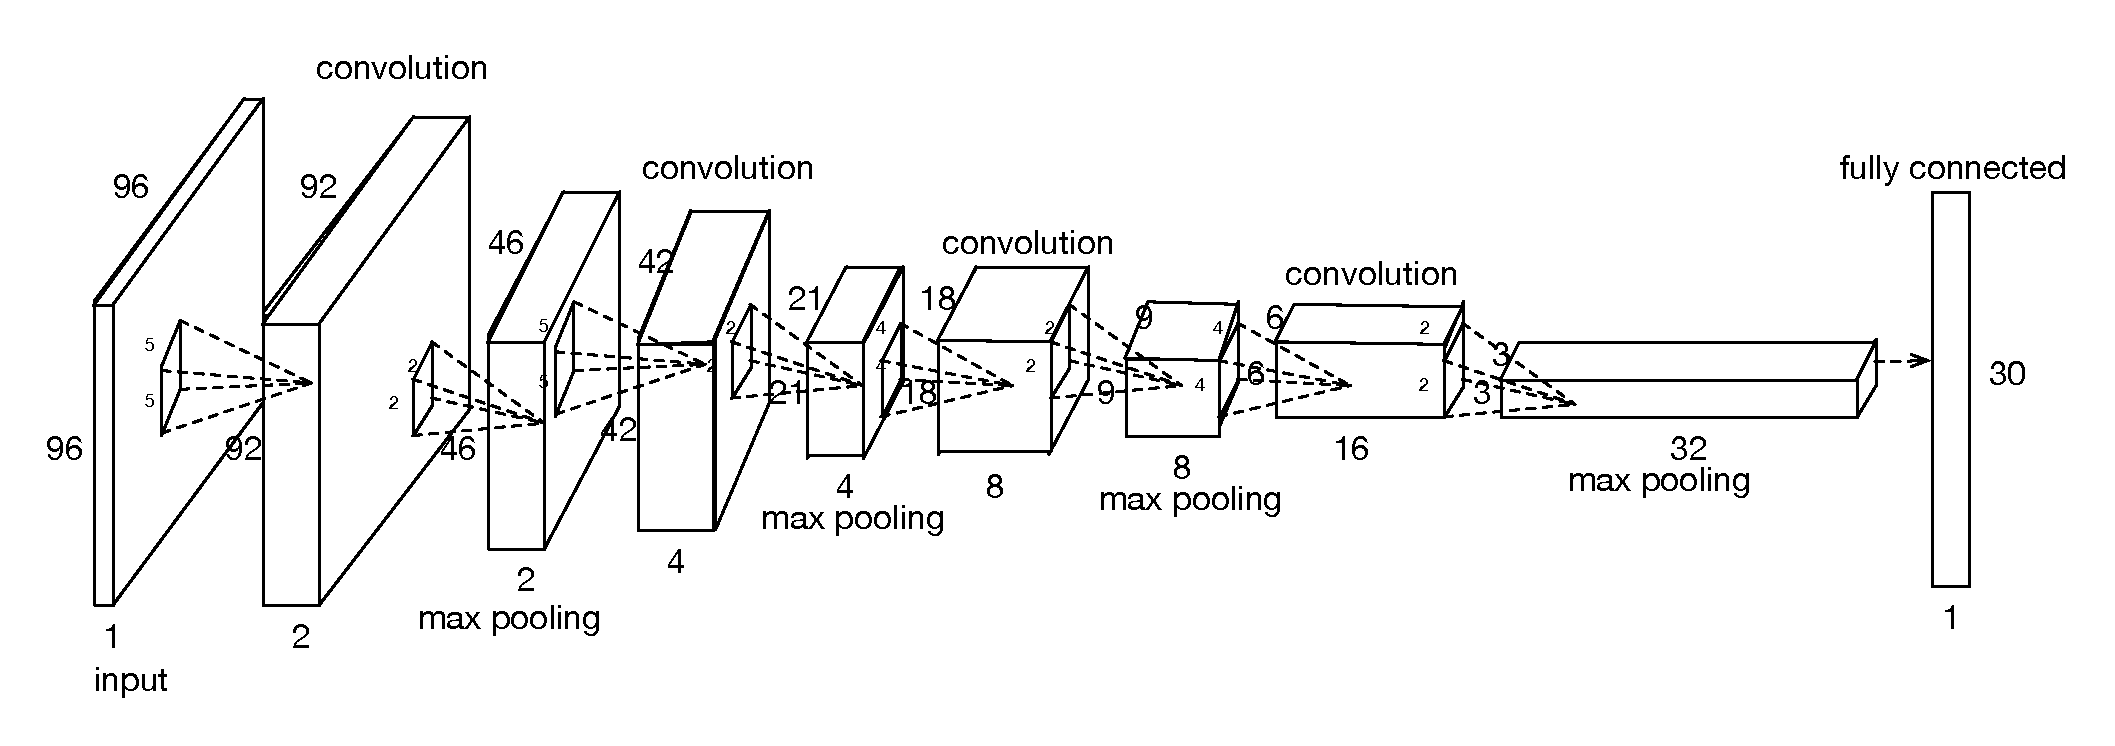
\includegraphics[width=0.8\linewidth]{figure1.eps}
   \caption{The structure of deep convolutional network F1. Sizes of input, convolution, and max pooling layers are illustrated by cuboids whose length, width, and height denote the number of maps, and the size of each map. Local receptive fields of neurons in different layers are illustrated by small squares in the cuboids}
\label{fig:single}
\end{figure}

The structure of level 2 networks are the same of the level 1 network. But level 2 networks only takes a subgraph of the original bitmap as the input. The subgraph is centered at the result from level 1 network. So level 1 network functions to narrow down the range. The struture of the whole cascaded network is shown in Figure 2. \\

\begin{figure}[htbp]
\centering
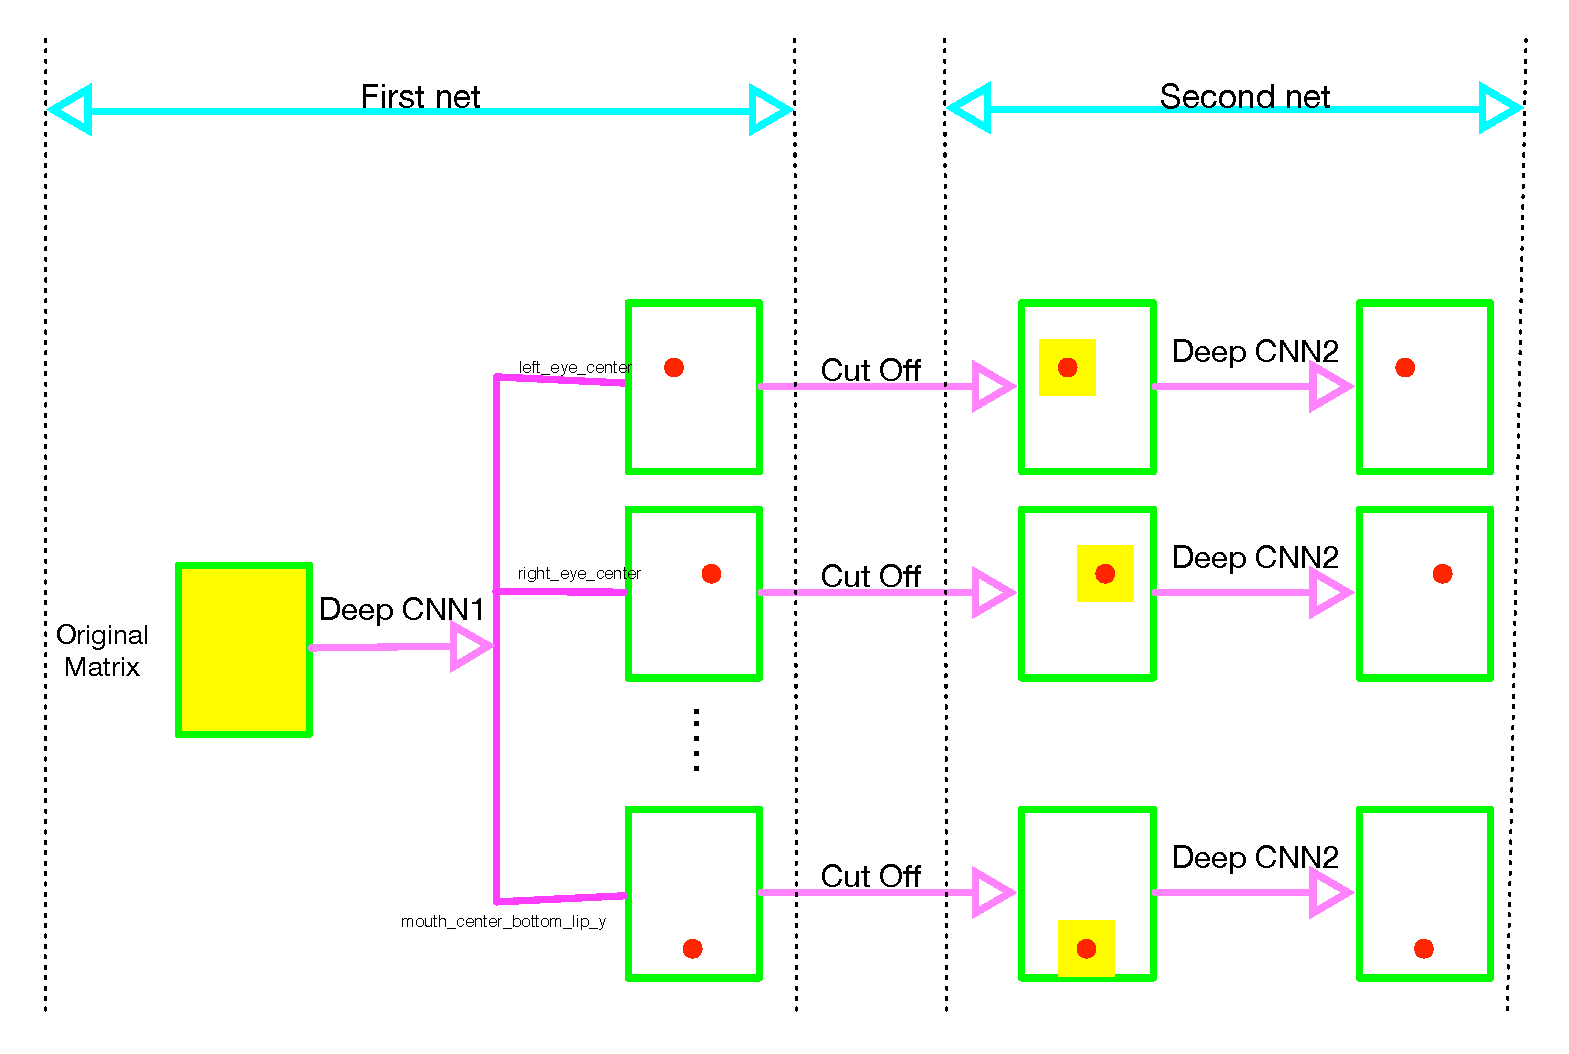
\includegraphics[width=0.8\linewidth]{figure2.eps}
   \caption{Two-level cascaded convolutional networks. The input is the bitmap matrix. The level 1 network takes the whole bitmap matrix as input, and outputs the predicted point coordinates. Then subgraphs centered at those coordinates are cut off for another deep convolutional network to get more precise answers.}
\label{fig:cascade}
\end{figure}

For the comparison, we build one mlp network(Figure 3) and one single convolutional network(just the one in Figure 1). Also we use another method of classification that maps the 96*96 matrix into a same size matrix. To make the aim matrix, we  convert the answer of training data into a 96*96 matrix with only the point nearest to the answer point is 1 and others 0. It goes very bad so we would not mention it in the Experiment part.

\begin{figure}[htbp]
\centering
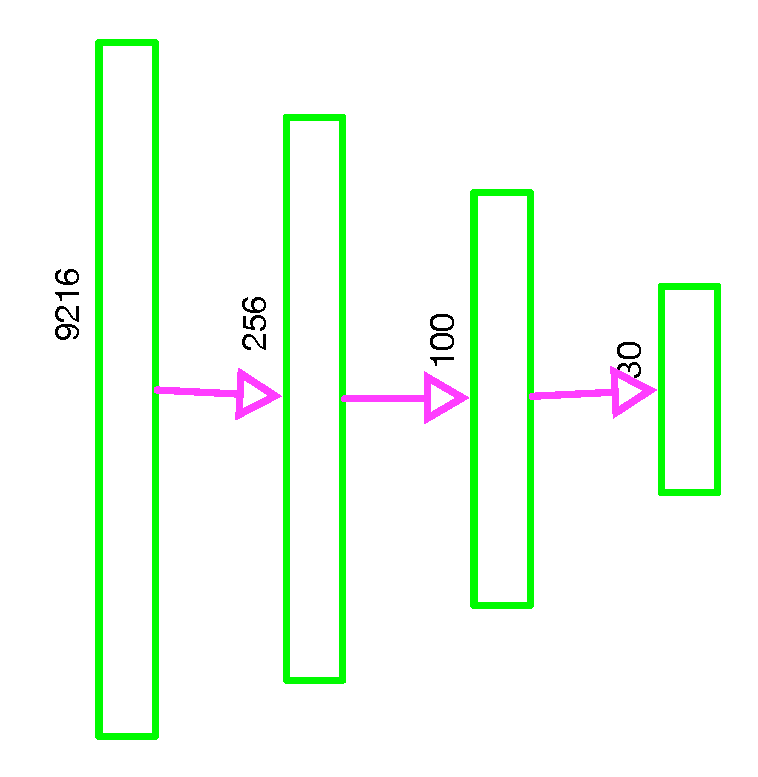
\includegraphics[width=0.8\linewidth]{MLP.eps}
   \caption{The structure of MLP layers.}
\label{fig:long}
\label{fig:onecol}
\end{figure}

\section{Experiment}

The size of data are shown in Table 1. \\
\begin{table}
\begin{center}
\begin{tabular}{|l|c|}
\hline
Point & number \\
\hline\hline
(level 1 network training data) & 2140\\
(level 2 network training data) & \\
left\_eye\_center & 7039 \\
right\_eye\_center & 7036 \\
left\_eye\_inner\_corner & 2271 \\
left\_eye\_outer\_corner & 2267 \\
right\_eye\_inner\_corner & 2268 \\
right\_eye\_outer\_corner & 2268 \\
left\_eyebrow\_inner\_end & 2270\\
left\_eyebrow\_outer\_end & 2225\\
right\_eyebrow\_inner\_end & 2270 \\
right\_eyebrow\_outer\_end & 2236 \\
nose\_tip & 7049 \\
mouth\_left\_corner & 2269 \\
mouth\_right\_corner & 2270 \\
mouth\_center\_top\_lip & 2275\\
mouth\_center\_bottom\_lip & 7016\\
(test data) & 1783 \\ 
\hline
\end{tabular}
\end{center}
\caption{Results.   Ours is better.}
\end{table}

In the training data, we use 400 samples for validation, and others for training. \\

\textbf{Single convolutional network} The cost and RMSE is shown in Figure 4 and 5. The prblem is that it gives almost same coordinates for one type of points, that is, a constant whatever the input bitmap is in the training data. Studying deep into the level 1 network, we find that the constant comes from the value of b in the last fully-connected layer, and the output of each individual convolutional layer is almost a matrix of zeros. Increasing the deviation standard in the initializing parameters part will make the shift around the constant large. As we train the 15 different types of points together, it is kind of difficult to satisfy all with the same kernal blocks in the convolutional layer, so it can easily drop into this local minimum. \\
%
\begin{figure}[htbp]
\centering
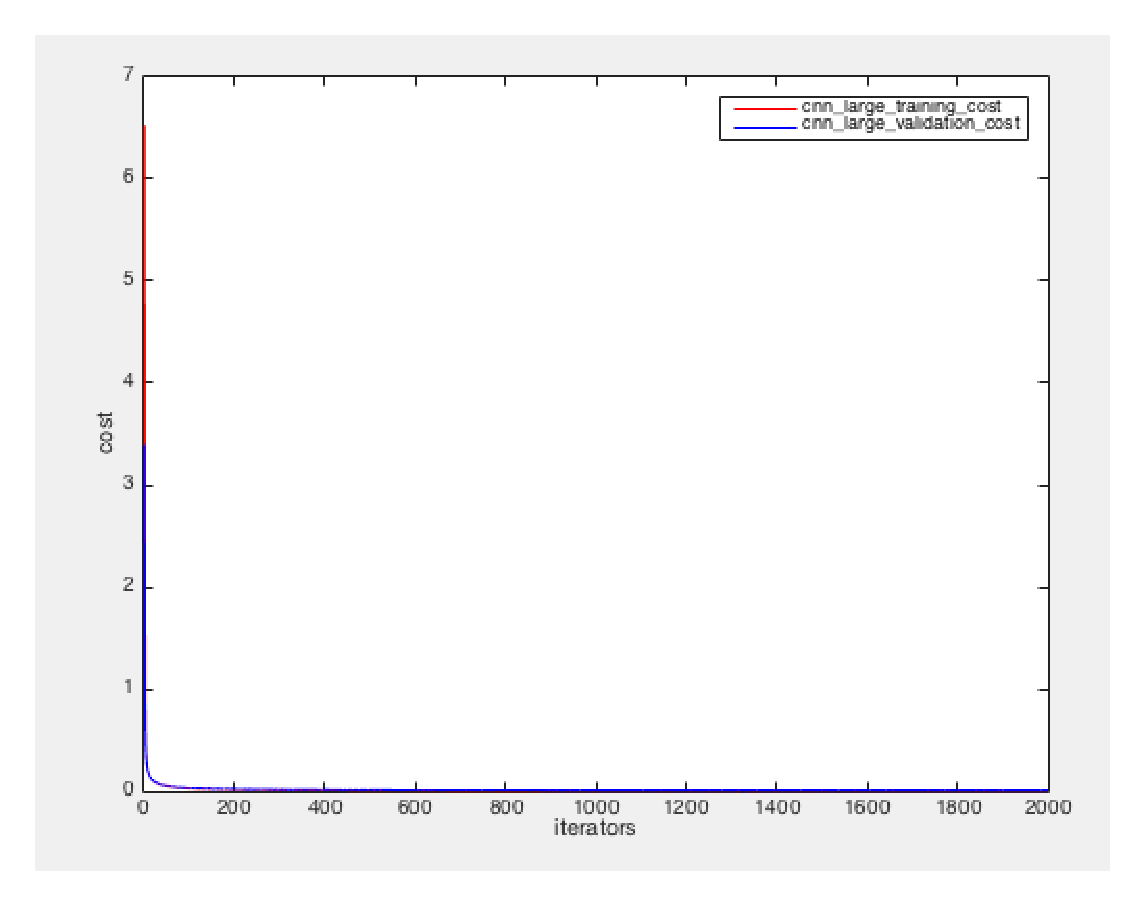
\includegraphics[width=0.8\linewidth]{cnn_large_cost.eps}
\caption{The accuracy of validation data in CNN.(10000 iters)}
\label{fig:long}
\label{fig:onecol}
\end{figure}

\begin{figure}[htbp]
\centering
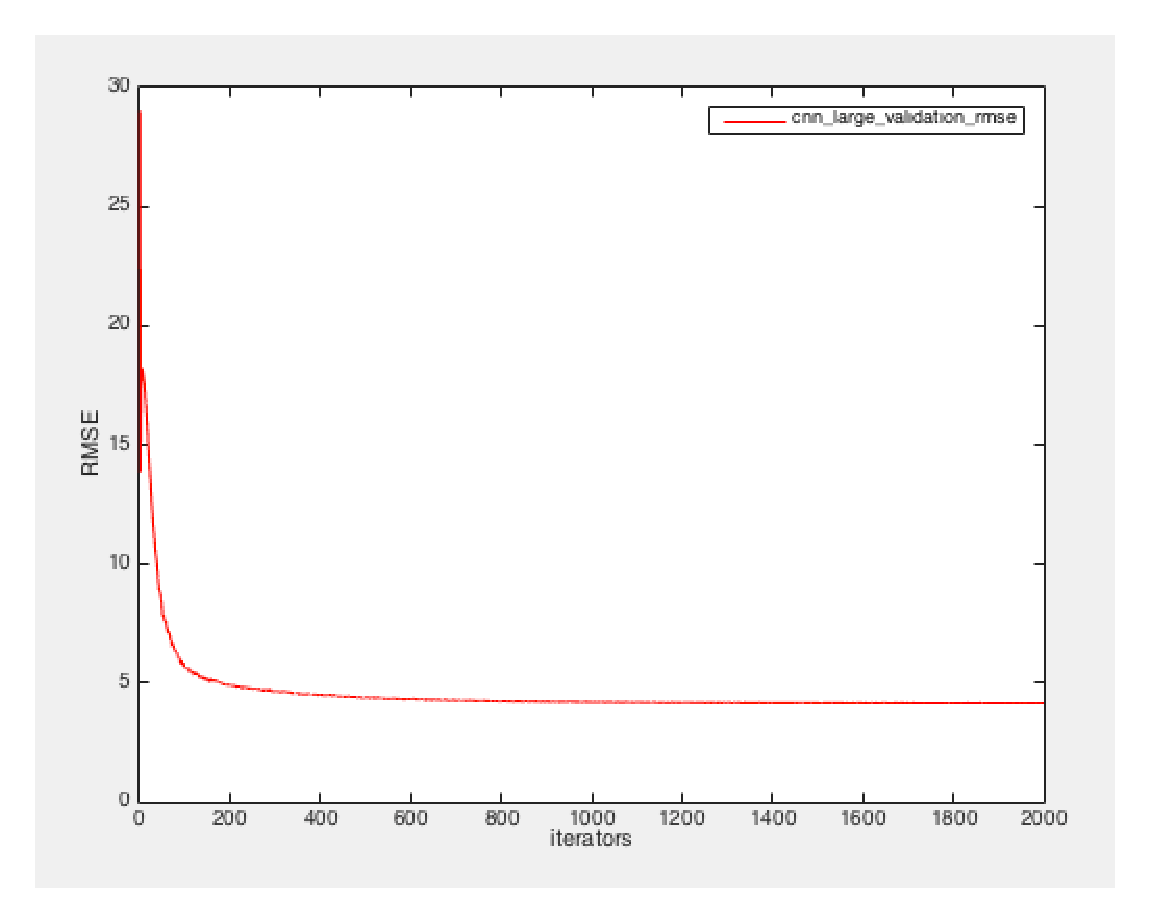
\includegraphics[width=0.8\linewidth]{cnn_large_rmse.eps}
\caption{The accuracy of validation data in CNN.(10000 iters)}
\label{fig:long}
\label{fig:onecol}
\end{figure}

Also we have tried to remove the shifting value b in the last fully-connected layer. And the result RMSE is $4.31$ in the test data after about 500 iterators. It is also a good choice. \\

\textbf{Cascaded convolutional network} From the knowledge of the single convolutional network we get that the level 1 network need not to be so deep, so we concentrate on the level 2 networks. As we can see in Table 1, we train the level 1 network with the common 2140 bitmaps with all 15 types of points given. Of course we almost get a contant coordinate for one type of points. And the distance between the real points and the contant coordinate is less than 25. So we make the size of subgraphs as 50*50. \\

The result is that it works well for the first several points with RMSE around 2.3. But it gets worse later with RMSE more than 3.5. \\

\textbf{MLP} MLP is a very simple network, but works well in this problem. The best result in all our submission is from MLP, with RMSE 3.73126, ranked 59 out of 127 teams. \\
We try MLP with and without dropout and the results are shown in Figure 6-9. The MLP without validation has a less RMSE, but the difference between training cost and validation cost is much large, meaning that the MLP without dropout can be easier to get overfitted.\\

\begin{figure}[htbp]
\centering
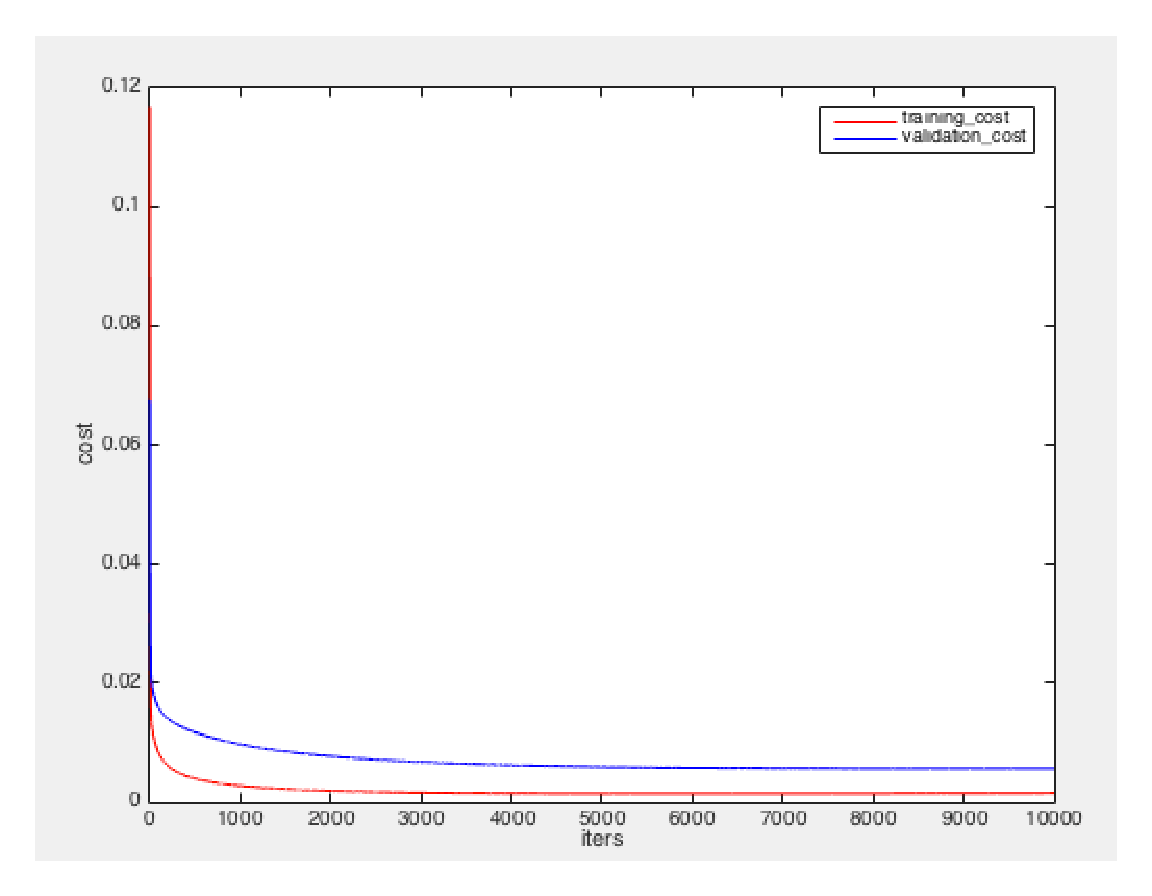
\includegraphics[width=0.8\linewidth]{MLP_cost.eps}
\caption{The cost of traing data and validation data in MLP.(10000 iters)}
\label{fig:long}
\label{fig:onecol}
\end{figure}

\begin{figure}[htbp]
\centering
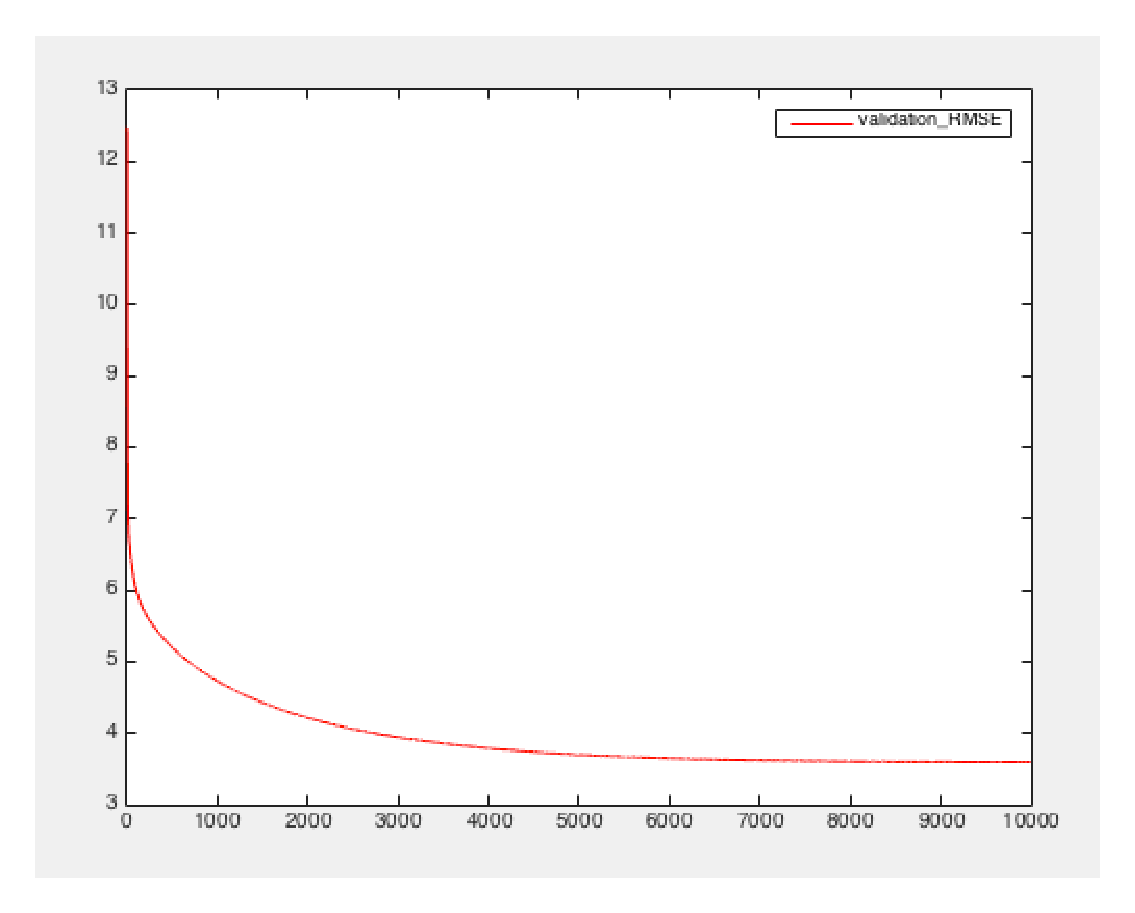
\includegraphics[width=0.8\linewidth]{MLP_RMSE.eps}
\caption{The accuracy of validation data in MLP.(10000 iters)}
\label{fig:long}
\label{fig:onecol}
\end{figure}

\begin{figure}[htbp]
\centering
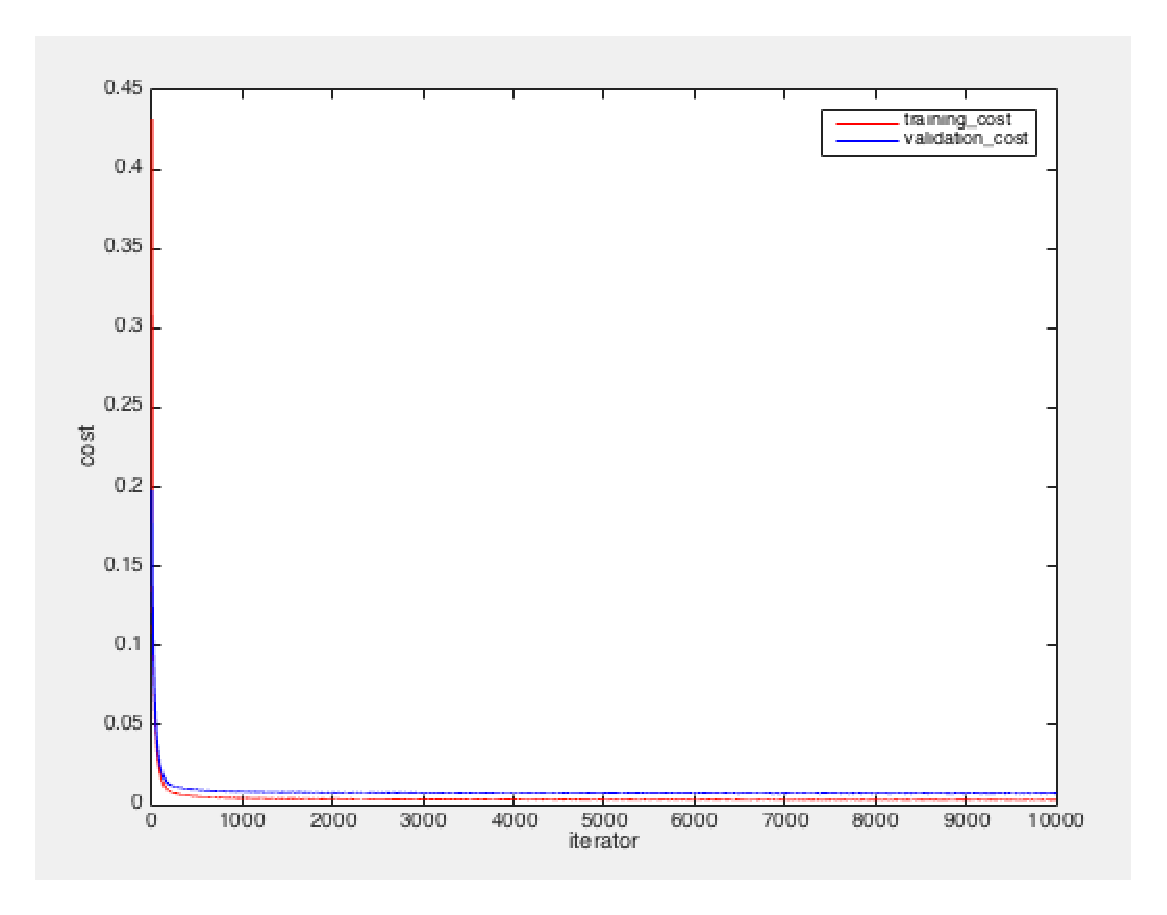
\includegraphics[width=0.8\linewidth]{mlp_dropout_cost.eps}
\caption{The accuracy of validation data in MLP.(10000 iters)}
\label{fig:long}
\label{fig:onecol}
\end{figure}

\begin{figure}[htbp]
\centering
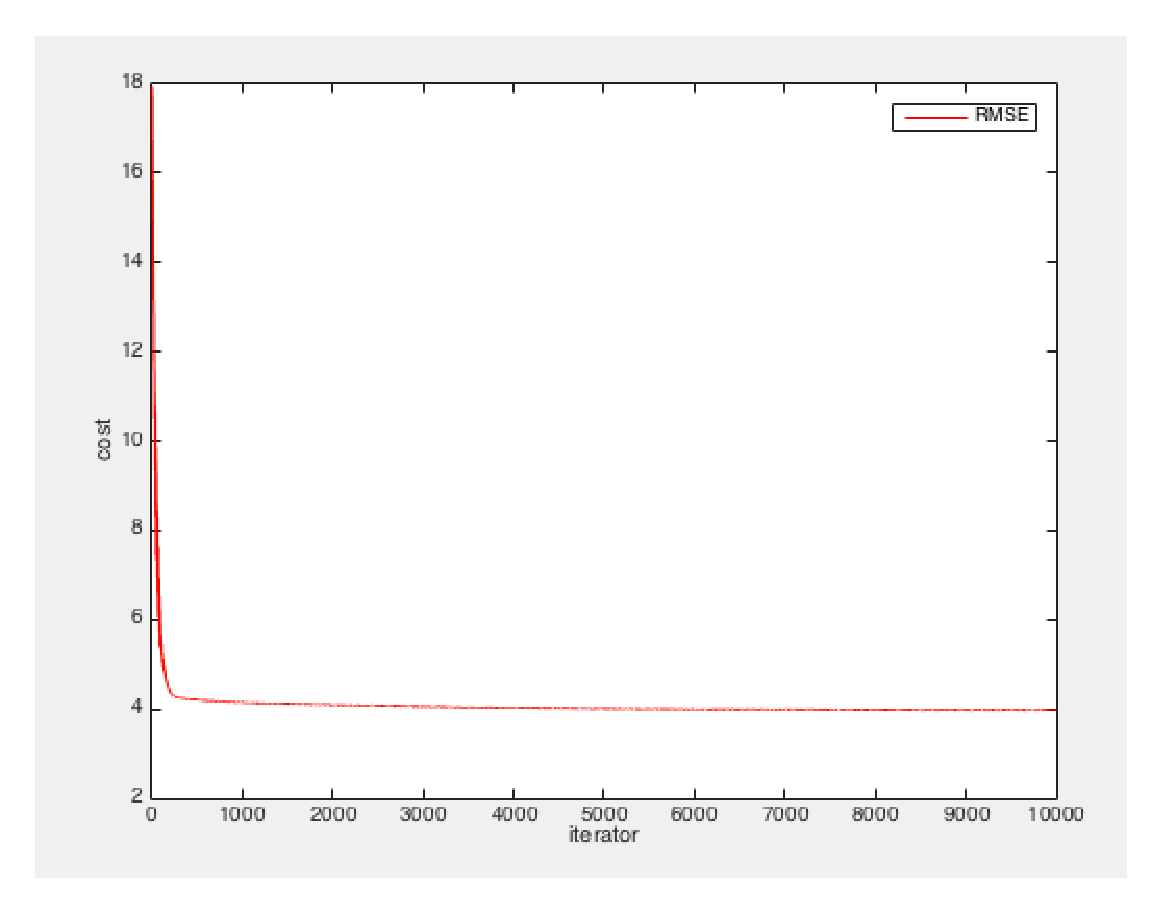
\includegraphics[width=0.8\linewidth]{mlp_dropout_rmse.eps}
\caption{The accuracy of validation data in MLP.(10000 iters)}
\label{fig:long}
\label{fig:onecol}
\end{figure}

\section{Conclusion}
In the above, we show our experiment result using several different neural net model to predict
location of facial key points. We stuck to a MSE of about 4.1 and have no truely improvement.

The convolutional net we used is considerably large, almost at the same scale for image-net classification
of \cite{krizhevsky2012imagenet}, but it even have not a single improvement compare to a very simple
three-layer MLP.

We have done many research on initialization method, and choose one that widely accepted as useful even when
training very deep neural net. But those state-of-art method can't event have a tiny improvement on my model
when training this task.

When faced with overfitting problem, we first implement regularization and lastly dropout. As we can observe,
dropout can dramatically reduce overfitting at the early stage of training. However when epochs went large,
it overfit as usual.

A simple MLP training for amazing 10000 epochs even have a better performance than a deep convolution layer.
And add dropout to MLP suddenly reduce its performance to the level of CNN.

As far as I'm concern, I have already tried the widely-accepted advanced techniques to my model, but they all
stuck to a certain point. I guess that the training dataset itself is not well labeled, and a convolution net
designed for accurate image processing can't fit all the errors in the label. While the MLP tend to overfit to
the training set, i.e. to the error labeled data. Since convolution net and dropout all reduce the overfitting,
so they can't achieve the same performance as the MLP.

{\small
\bibliographystyle{ieee}
\bibliography{egbib}
}

\end{document}
